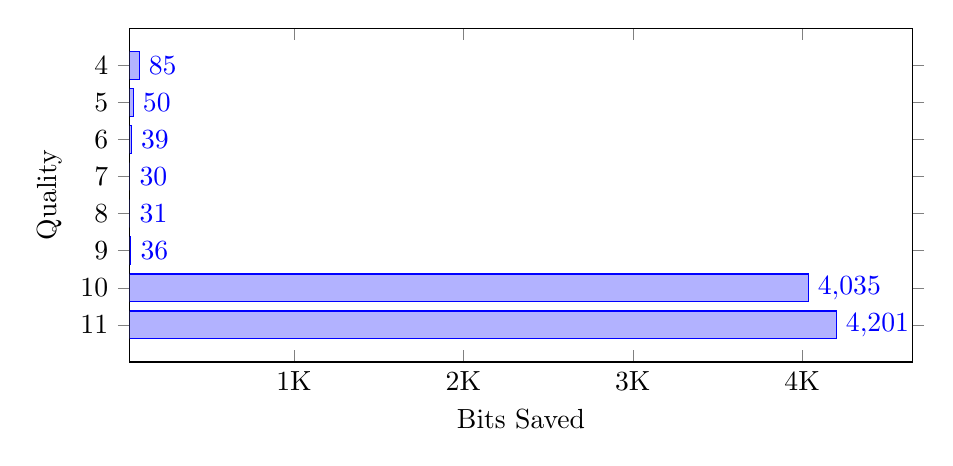
\begin{tikzpicture}
\begin{axis}[
	width = 0.95\textwidth,
	height = 0.8*\axisdefaultheight,
	xbar,
	xmax = 4650,
	xtick = {0, 1000, 2000, 3000, 4000},
	xticklabels = {$0$K, $1$K, $2$K, $3$K, $4$K},
	y dir = reverse,
	ytick = data,
	scaled ticks = false,
	enlarge x limits = {abs = 0},
	enlarge y limits = {abs = 1},
	nodes near coords,
	nodes near coords align = {horizontal},
	xlabel = Bits Saved,
	ylabel = Quality
]
\addplot coordinates {
	(85, 4)
	(50, 5)
	(39, 6)
	(30, 7)
	(31, 8)
	(36, 9)
	(4035, 10)
	(4201, 11)
};
\end{axis}
\end{tikzpicture}